\section{Οικογένειες Αθροιστών}
Σε αυτή την ενότητα Θα παρουσιαστούν κάποιες βασικές ομάδες αθροιστών με βάση την αρχιτεκτονική τους.


\subsection{Διάδοσης Κρατουμένου}
Αθροιστής Διάδοσης Κρατουμένου ή Ripple-Carry Adder (RCA) είναι ο πιο απλός αθροιστής και το σχηματικό του είναι στην εικόνα \ref{IntegerAdderSchematic}. Παρατηρούμε πως για να υπολογιστεί το sum[1] δηλαδή το δεύτερο λιγότερο σημαντικό ψηφίο του αθροίσματος πρέπει πρώτα να υπολογιστεί το c\_out του προηγούμενου πλήρη αθροιστή , αντίστοιχα για το τρίτο πρέπει να υπολογιστεί πρώτα το c\_out[0] έπειτα από τον δεύτερο πλήρη αθροιστή να υπολογιστεί το c\_out[1] με είσοδο στο c\_in το το c\_out[0] δηλαδή το c\_out του προηγούμενου . Συμπεραίνουμε λοιπόν πως κάθε FA δεν λειτουργεί παράλληλα με τα υπόλοιπα αλλά υπάρχει μια χρονική καθυστέρηση για να λάβει την σωστή είσοδο c\_in . Αποτέλεσμα αυτού είναι πως στην χειρότερη περίπτωση , δηλαδή στην περίπτωση που το c\_in επηρεάζει άμεσα την τιμή του c\_out του αθροιστή , υπάρχει γραμμική αύξηση της καθυστέρησης με το μήκος του .
Για παράδειγμα έχοντας έναν δυαδικό αθροιστή 8 ψηφίων και εισάγοντας τους αριθμούς Α = 00000000 και Β = 11111111 και c\_in = 0 θα πάρουμε έξοδο sum = 11111111 και c\_out = 0 . Αν κρατώντας όλες τις εισόδους σταθερές και αλλάζοντας μόνο την Α σε 00000001 δηλαδή το Α[0]=1 τότε το αποτέλεσμα θα είναι sum=00000000 και c\_out = 1 . 
\par
Η περίπτωση που περιγράφηκε ανήκει στις χειρότερες περιπτώσεις διότι 


\subsection{Παράλειψής Κρατουμένου}
Για κάθε ψηφίο του αριθμού Α και Β ορίζονται δυο ακόμα στοιχεία , αυτά που παράγουν κρατούμενο ανεξάρτητα του κρατουμένου εισόδου και θα καλούνται generate και αυτά που διαδίδουν κρατούμενο και ονομάζουμε propagate . Οι εξισώσεις είναι αντίστοιχα :
\begin{equation}
\begin{split}
    g_i &= A_i * B_i  \\
    p_i &= A_i \oplus B_i 
\end{split}
\end{equation}
ή
\begin{equation*}
    p_i = A_i + B_i
\end{equation*}
Όταν έχουμε $g_i=1$ τότε γνωρίζουμε πως ο συγκεκριμένος πλήρης αθροιστής παράγει κρατούμενο εξόδου . Σε αντίθεση με την συνάρτηση εξόδου του c\_out του Full-Adder η συνάρτηση του generate είναι πιο απλή καθώς αποτελείται από μόνο μια πύλη AND άλλα δεν εγγυάται αν θα υπάρχει κρατούμενο εισόδου ή όχι .Δηλαδή αν $g_i=1$ τότε και $c\_out_i=1$ χωρίς όμως να ισχύει το αντίθετο. 

%-----------------
Είναι μια υλοποίηση αθροιστή που βελτιώνει την καθυστέρηση του αθροιστή διάδοσης κρατουμένου με έναν απλό τρόπο αλλά όχι αρκετά αποτελεσματικό σε σχέση με άλλες αρχιτεκτονικές. 
Η χείριστη περίπτωση παρουσιάζεται όταν σε έναν ripple-carry όταν το propagate στοιχείο είναι αληθές για κάθε ζευγάρι ψηφίων (A\_i B\_i) .
Ορίζοντας τον propagate όρο ως το XOR των Α\_i B\_i 
Όταν όλοι οι όροι propagate είναι αληθείς τότε το κρατούμενο εισόδου προσδιορίζει το κρατούμενο εξόδου .
Παίρνοντας κάθε όρο propagate και εισάγοντας τον σε μια n-εισόδων πύλη AND ορίζουμε τον όρο select το οποίο οδηγεί την είσοδο επιλογής ενός πολυπλέκτη 2-σε-1 ,όπου η έξοδος του είναι το c\_out του αθροιστή , και όταν το select είναι εληθες τότε επιλέγεται το c\_in αλλιώς το c\_n .
%ΣΗΜΑ 
\begin{equation}
\begin{split}
    p_i &= A_i \oplus B_i \\
    select &= p_0 * p_1 * ... * p_{n-1} \\
    c\_out &= select\ ?\ c\_in\ :\ c_{n-1} % c_n-1 = c_out 
\end{split}
\end{equation}
%ΟΡΙΣΕ ΑΝ ΘΑ ΛΕΣ ΤΟ ΚΡΑΤΟΥΜΕΝΟ ΕΙΣΟΔΟΥ C_0 ‘H C_-1
Η βελτιστοποίηση της χείριστης περίπτωσης επιτυγχάνεται με την χρήση πολλαπλών αθροιστών παράβλεψης κρατουμένου για να δομήσουν έναν block-carry-skip αθροιστή. Στην αντίθετή περίπτωση η καθυστερήσεις είναι ίδιες με αυτές του ripple-carry.
Ο αριθμός των εισόδων της πύλης AND για τον υπολογισμό του select είναι ίσος με τον μήκος του αθροιστή με αποτέλεσμα ένας αθροιστής μεγάλου μήκους να καθίσταται μη πρακτικός εφόσον οδηγεί σε επιπλέον καθυστερήσεις, διότι η πύλη AND πρέπει να κατασκευαστεί σαν ένα δέντρο.   
%-----------------



\subsection{Επιλογής κρατουμένου}
Ο αθροιστής επιλογής κρατουμένου ή Carry-Sellect Adder υλοποιείται με τον εξής τρόπο :
\begin{itemize}
  \item Έχουμε δυο αθροιστές ιδίου μήκους και εκτελούν τις ίδιες προσθέσεις με την διαφορά πως ο ένας έχει ως κρατούμενο εισόδου 0 και ο άλλος 1.
  \item Το κρατούμενο εισόδου του αθροιστή οδηγεί την είσοδο επιλογής ενός πολυπλέκτη με είσοδο τα αποτελέσματα των δυο αθροιστών που προαναφέρθηκαν.
  \item Ανάλογα με την κατάσταση του κρατουμένου εισόδου επιλέγεται και το σωστό αποτέλεσμα στην έξοδο.
\end{itemize} 









\subsection{Πρόβλεψης Κρατουμένου}
Σε αντίθεση με τις προηγούμενες τακτικές βελτίωσης της άθροισης ο Αθροιστής Πρόβλεψης Κρατουμένου ή Carry-Lookahead Adder (CLA) βελτιώνει την ταχύτητα μειώνοντας τον χρόνο υπολογισμού κάθε ενδιάμεσου κρατουμένου καθώς και του τελικού c\_out .
Αυτή η αρχιτεκτονική υλοποιείται με τον παρακάτω τρόπο :
\begin{itemize}
    \item Υπολογίζονται, για κάθε ζεύγος ( $A_i$ , $B_i$ ) δύο σήματα, το ένα αληθεύει 
    όταν το ζεύγος μπορεί να διαδώσει το κρατούμενο που εξάγει το προηγούμενο ζεύγος 
    και το άλλο αληθεύει όταν το παρόν ζευγάρι παράγει κρατούμενο ανεξαρτήτως το 
    αν θα έχει κρατούμενο εισόδου ή όχι. Τα σήματα αυτά θα ονομαστούν propagate ή p
    και generate ή g, αντίστοιχα. 
    \item Συνδυάζοντας αυτά τα σήματα δίνεται η δυνατότητα να προσδιοριστεί ταχύτερα αν ένα τμήμα ζευγών ψηφίων πρόκειται να διαδώσει ή να παράξει ένα κρατούμενο .
\end{itemize}


Για παράδειγμα σε έναν αθροιστή των τεσσάρων bits η διάδοση του κρατουμένου εισόδου από το πρώτο έως το τελευταίο bit εξαρτάται από την ομάδα διάδοσης κρατουμένου ή Group Propagate (P). Επίσης η παραγωγή κρατουμένου εξαρτάται από την ομάδα παραγωγής κρατουμένου ή Group Generate (G) των τεσσάρων ζευγών. Για το P είναι εύκολο να βρούμε την συνάρτηση bool του εφόσον το έχουμε συναντήσει και στις παραπάνω ομάδες αθροιστών , αντίθετα το G είναι πιο περίπλοκο. 

\begin{figure}[H]
\centering
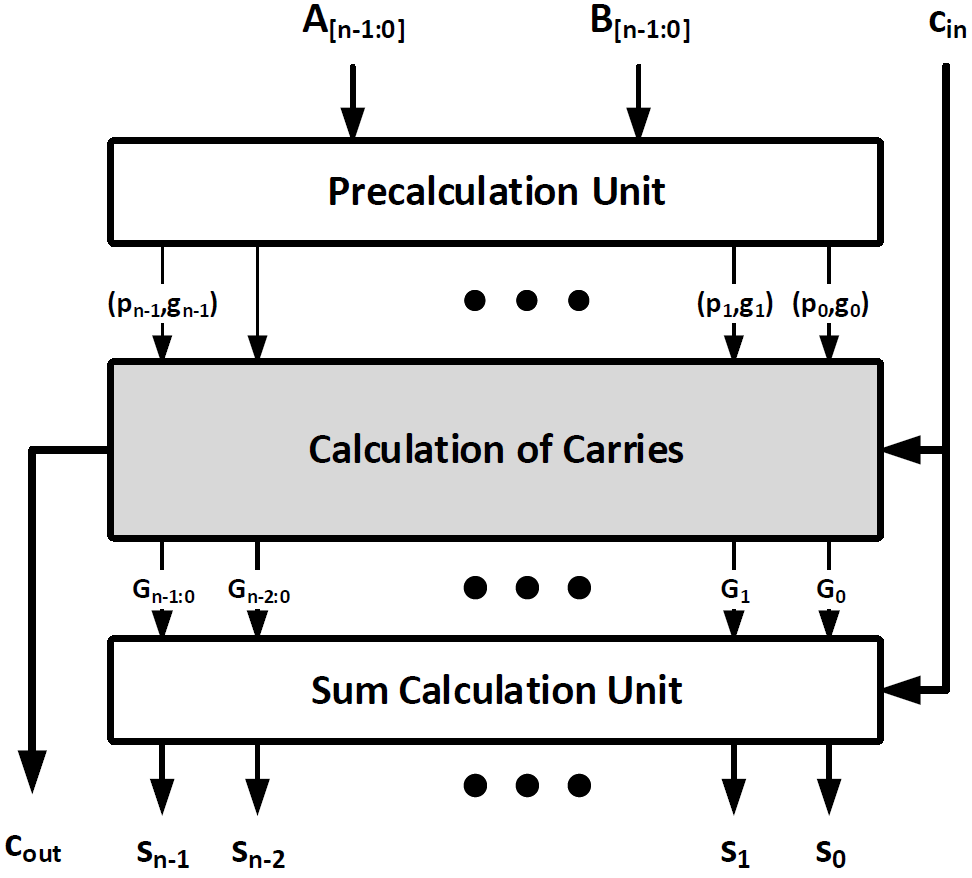
\includegraphics[width=\textwidth]{Pictures/CLA_Architecture.png}
\caption{CLA Architecture}
\label{cla_architecture}
\end{figure}

\textcolor{red}{Αναλυση της εικόνας}